\documentclass{article}

% Language setting
% Replace `english' with e.g. `spanish' to change the document language
\usepackage[french]{babel}
\usepackage[fleqn]{amsmath} % Aligner les équations à gauche


% Set page size and margins
% Replace `letterpaper' with`a4paper' for UK/EU standard size
\usepackage[letterpaper,top=2cm,bottom=2cm,left=3cm,right=3cm,marginparwidth=1.75cm]{geometry}

% Useful packages

\usepackage{amsmath}
\usepackage{graphicx}
\usepackage{subcaption}
\usepackage[colorlinks=true, allcolors=blue]{hyperref}

\title{TD 1 - Optique géométrique }
\author{IPESUP - PC }
\date{DATE }

\begin{document}
\maketitle



\section{Rappels de cours}

\begin{itemize}
  \item Loi de Snell-Descartes pour la réflexion : lors d'un changement de milieu (d'indice $n_1$ à $n_2$), le rayon réfracté appartient au plan formé par le rayon incident et la normale au point d'incidence. Les angles $i$ et $r$ entre la \textbf{normale} et le \textbf{point d'incidence} respectent la relation suivante $\frac{\sin(i)}{\sin(r)} = \frac{n_2}{n_1}$
  \item Relation de conjugaison de Descartes: $\frac{1}{\overline{OA'} } - \frac{1}{\overline{OA} } = \frac{1}{f'}$. Attention aux signes ! 
  \item Relation de Newton : $\overline{F'A'} \times \overline{FA} = -f'^2$
\end{itemize}
\section{Chemins optiques}

La lentille (L) est en verre d'indice $n$ et de centre optique $O$.
Elle a une épaisseur $e$ au niveau du centre optique. 
Soit $f'$ la distance focale de la lentille et $n_{air}$ l'indice optique de l'air.
Soient $M$ et $M'$ deux point de l'espace dont les coordonnées sont respectivement $(x,0)$ et $(x',y')$.
On place une source de lumière $S$ devant la lentille sur l'axe $(Ox)$. 
\begin{enumerate}
  \item On suppose que $OS=f'$. Représenter le schéma de la situation et construire les rayons issus de $S$ qui parviennent en $M$ et $M'$. Exprimer $(SM)$ et $(SM')$ les chemins optiques. 
  \item Même question si $OS=\frac{3f'}{2}$.
\end{enumerate}




\begin{figure}[h]
  \centering
  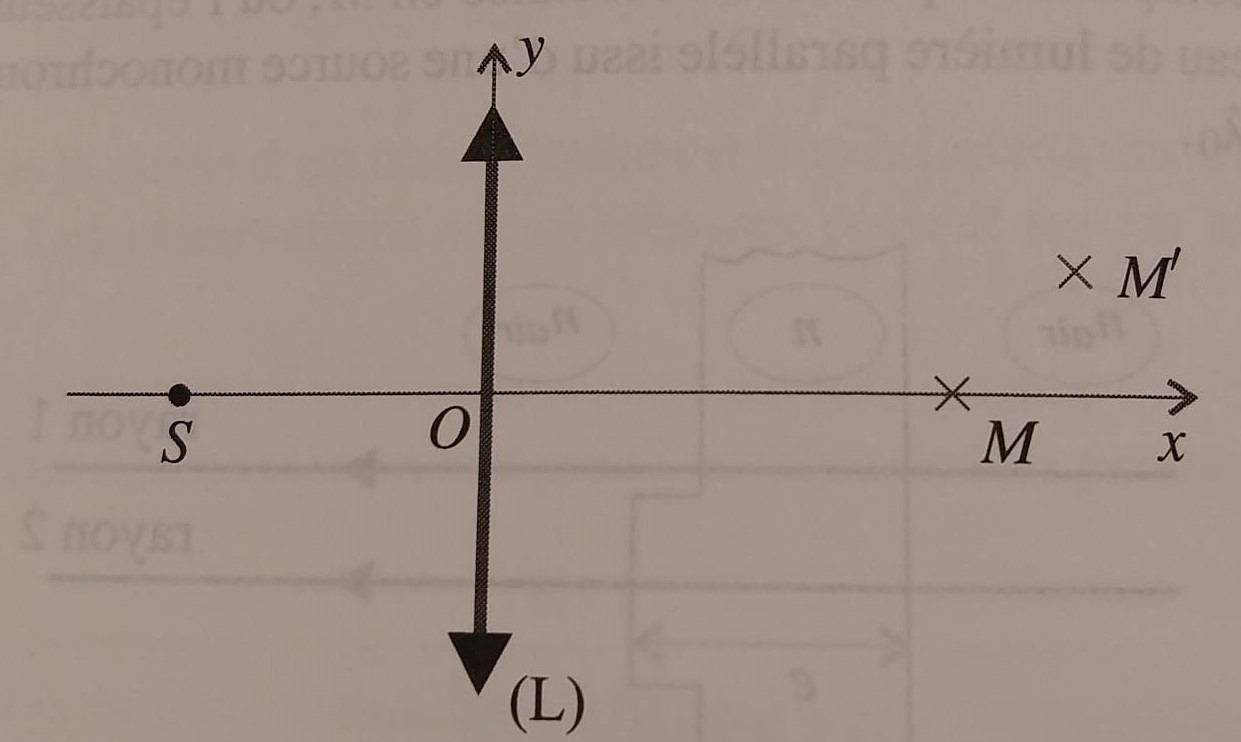
\includegraphics[width=0.3\textwidth]{exercice 1.jpg}
  \label{fig:ex}
    \caption{Schéma de la lentille}
\end{figure}


\section{Modèle d'une cavité}

On modélise une cavité optique par une suite de lentilles convergentes identiques de focale $f'$, coaxiales, et séparées d'une distance $a$. 
La lentille $n$ est frapée au point d'abscisse $y_n$ par un rayon lumineux.
L'angle entre l'horizontale et le rayon lumineux est noté $\alpha_n$ et est compté positivement dans le sens direct. 
\begin{enumerate}
  \item Déterminer deux relations de réccurence entre $y_{n+1}$ et $y_n$, $\alpha_{n+1}$ et $\alpha_n$ puis en déduire une relation d'ordre 2 sur les $y_n$. 
  \item A quelle condition sur $a$ et $f$ le dispositif est-il intéressant ? 
  \item Résoudre le problème dans le cas où $a=2f$.
\end{enumerate}

\begin{figure}[h!]
  \centering
  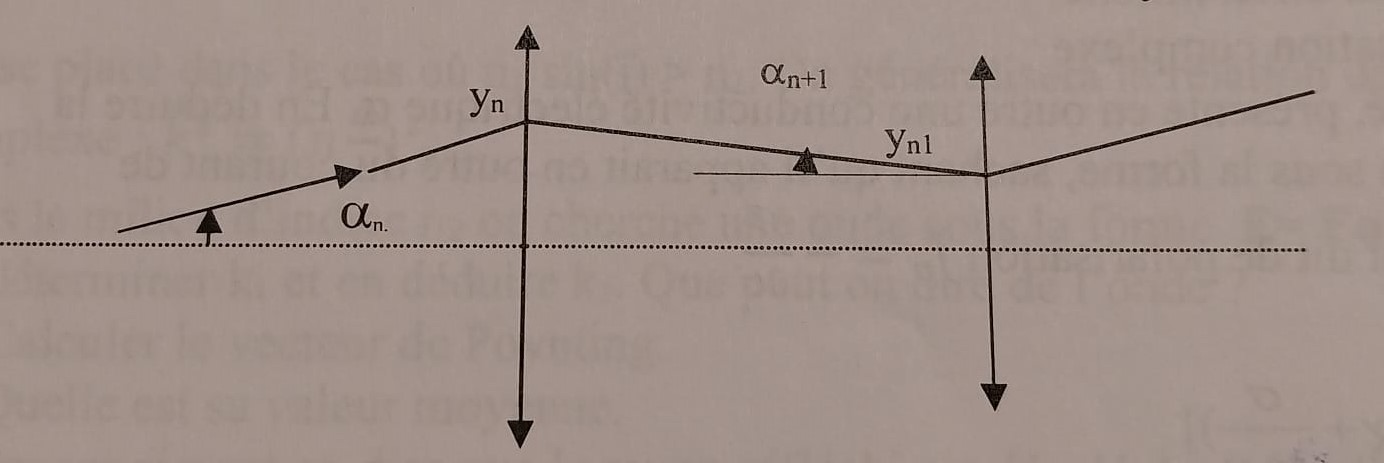
\includegraphics[width=0.4\textwidth]{exercice 2.jpg}
    \caption{Schéma de la cavité}
\end{figure}
\newpage
\section{Fibre optique}

On considère une fibre optique orientée selon l'axe $(Oz)$ dont le milieu est d'indice variable $n(r)=n_0 \sqrt{1-(\frac{kr}{a})^2}$ et dont la gaine est d'indice $n_G$. 
\begin{enumerate}
  \item Déterminer $k$ pour avoir continuité de l'indice. 
  \item Pourquoi peut-on se placer dans le plan $(Ozx)$ ? 
  \item On considère un rayon incident sur une strate $r=cte$ d'angle d'incidence $i$. Montrer qu'on a alors $n(r)sin(i) = C$. 
  \item En déduire que $(\frac{dr}{dz})^2 = A n(r)^2 - 1$, avec $A$ une constante à déterminer. 
  \item Déterminer $r(z)$ l'équation de la trajectoire d'un rayon lumineux. 
\end{enumerate}


\begin{figure}[h!]
  \centering
  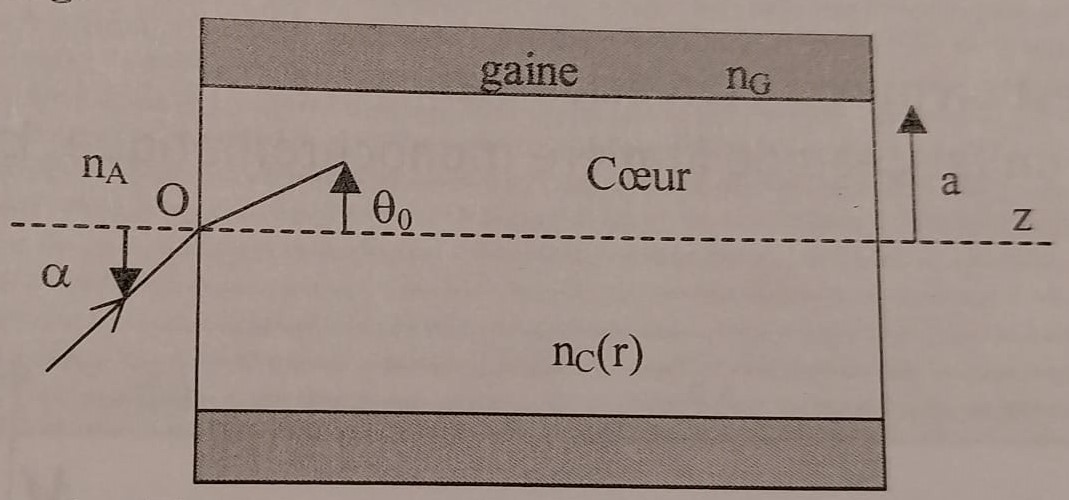
\includegraphics[width=0.4\textwidth]{exercice 3.jpg}
    \caption{Schéma de la gaine}
\end{figure}

\end{document}

